\documentclass[%handout %handout erstellen
]{beamer}
\usepackage[orientation=landscape,size=custom,width=16,height=9,scale=0.5,debug]{beamerposter}

\usepackage[utf8]{inputenc}
\usepackage[naustrian]{babel}
\usepackage{color}
\usepackage{url}
\usepackage{lmodern}
\usepackage{listings}
\usepackage{subfigure}
\usepackage[font=footnotesize,labelformat=empty]{caption}

\hypersetup{pdftitle={\inserttitle},
  pdfsubject={\inserttitle},
  pdfauthor={\insertauthor},
  pdfkeywords={\inserttitle},
  pdfpagelabels={false},
%  pdfpagemode={FullScreen}
}
\definecolor{darkred}{rgb}{.7,0,0}
\definecolor{darkblue}{rgb}{0,0,.5}
\definecolor{darkgreen}{rgb}{0,.5,0}

\lstset{
  extendedchars=\true,
  language=Bash,
  frame=none,
  captionpos=b,
  basicstyle={\fontsize{9}{9}\ttfamily},
  tabsize=2,
  keywordstyle=\color{darkred},
  commentstyle=\color{darkblue},
  stringstyle=\color{darkgreen}
}

\usetheme{Singapore}
%\progressbaroptions{headline=none,frametitle=picture-section,imagename=img/logo.jpg}
%\setbeamercovered{transparent}  %halbtransparente uebergaenge
%\beamertemplatenavigationsymbolsempty 	%keine nav-symbole

\mode<handout>{
  \setbeameroption{show notes}  %notizen nur bei handouts
  \usepackage{pgfpages}
  \pgfpagesuselayout{2 on 1}[a4paper, border shrink=5mm]
%  \pgfpagesuselayout{4 on 1}[a4paper, landscape, border shrink=5mm]
  \pgfpageslogicalpageoptions{1}{border code=\pgfusepath{stroke}}
  \pgfpageslogicalpageoptions{2}{border code=\pgfusepath{stroke}}
%  \pgfpageslogicalpageoptions{3}{border code=\pgfusepath{stroke}}
%  \pgfpageslogicalpageoptions{4}{border code=\pgfusepath{stroke}}
}

\title{Git Workshop}
\subtitle{VALUG - 8. April 2011}
\author[Florian Preinstorfer, Wolfgang Silbermayr]{Florian Preinstorfer, Wolfgang Silbermayr}
\date[valug - 08.04.2011]{08.04.2011}
\titlegraphic{

\includegraphics[height=.7cm]{img/git-logo-wikipedia-export}\\
\vspace{0.2cm}

\includegraphics[height=0.5cm]{img/by-sa}
}

\begin{document}
\frame[plain]{\titlepage}

\begin{frame}{Inhalt}
  \tableofcontents[pausesections]
\end{frame}

\section{Versionskontrolle}

\begin{frame}
  \tableofcontents[currentsection]
\end{frame}

\begin{frame}{Was ist Versionskontrolle}
\end{frame}

% vim: tabstop=2 expandtab shiftwidth=2 softtabstop=2 autoindent

\section{Einstieg in git}

\begin{frame}
  \tableofcontents[currentsection]
\end{frame}

\begin{frame}{Installation}
  \begin{itemize}
    \item Linux:
    \begin{itemize}
      \item Debian, Ubuntu: \texttt{[sudo] apt-get install \textit{git-core}}
      \item Arch: \texttt{[sudo] pacman -S \textit{git}}
    \end{itemize}
    \item Windows:
    \begin{itemize}
      \item MySysGit: \url{http://code.google.com/p/msysgit}
      \item TortoiseGit: \url{http://code.google.com/p/tortoisegit}
    \end{itemize}
    \item Mac:
    \begin{itemize}
      \item Git for OS X: \url{http://code.google.com/p/git-osx-installer}
    \end{itemize}
  \end{itemize}
\end{frame}

\begin{frame}[fragile]{initiale Konfiguration}
  \begin{itemize}
    \item Identität festlegen:
    \begin{lstlisting}
$ git config --global user.name "John Doe"
$ git config --global user.email johndoe@example.com
    \end{lstlisting}
    \item Editor festlegen (optional):
    \begin{lstlisting}
$ git config --global core.editor whatever
    \end{lstlisting}
    \end{itemize}
\end{frame}

\begin{frame}{Die möglichen Zustände einer Datei}
  \begin{columns}
    \begin{column}{0.45\textwidth}
      \begin{figure}
        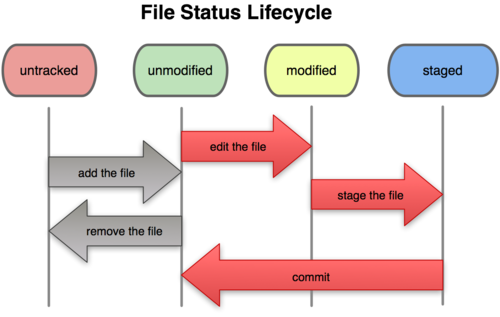
\includegraphics[width=\textwidth]{img/file_lifecycle}
        \caption[format=empty]{Quelle: \url{http://progit.org}}
      \end{figure}
    \end{column}
    \begin{column}{0.65\textwidth}
      \begin{itemize}
        \item Nicht versioniert (\textbf{untracked})
        \item Versioniert, aber unverändert (\textbf{unmodified})
        \item Versioniert und verändert (\textbf{modified})
        \item Versioniert, verändert und in der „staging area“ (\textbf{staged})
      \end{itemize}
    \end{column}
  \end{columns}
\end{frame}

\begin{frame}[fragile]{Die ersten Schritte}
  \begin{columns}
    \begin{column}{0.65\textwidth}
      \begin{itemize}
        \item Initialisieren eines git Repositories
        \begin{lstlisting}
$ cd meinprojekt
$ git init
        \end{lstlisting}
        \item Dateien zur „staging area“ hinzufügen
        \begin{lstlisting}
$ git add <file>
        \end{lstlisting}
        \item Änderungen der „staging area“ committen
        \begin{lstlisting}
$ git commit -m 'initial commit'
        \end{lstlisting}
      \end{itemize}
    \end{column}
    \begin{column}{0.35\textwidth}
      \begin{figure}
        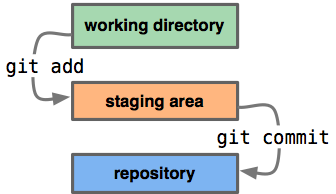
\includegraphics[width=\textwidth]{img/addcommit}
        \caption[format=empty]{Quelle: \url{http://whygitisbetterthanx.com}}
      \end{figure}
    \end{column}
  \end{columns}
\end{frame}

\begin{frame}[fragile]{Status betrachten}
  \begin{itemize}
    \item Den aktuellen Status des Repositories betrachten
    \begin{lstlisting}
$ git status
    \end{lstlisting}
  \end{itemize}
  \begin{lstlisting}[language=diff,frame=single,caption={Ausgabe von git status}]
# On branch master
# Changes to be committed:
#   (use "git reset HEAD <file>..." to unstage)
#
# %*\textcolor{darkgreen}{modified:   LICENSE}*)
#
# Changes not staged for commit:
#   (use "git add <file>..." to update what will be committed)
#   (use "git checkout -- <file>..." to discard changes in working dir)
#
# %*\textcolor{darkred}{modified:   notes.txt}*)
#
# Untracked files:
#   (use "git add <file>..." to include in what will be committed)
#
# %*\textcolor{darkred}{test.txt}*)
  \end{lstlisting}
\end{frame}

\begin{frame}[fragile]{Änderungen betrachten}
  \begin{itemize}
    \item Änderungen im Arbeitsverzeichnis betrachten
    \begin{lstlisting}
$ git diff
    \end{lstlisting}
    \item Änderungen betrachten, die sich bereits in der „staging area“ befinden
    \begin{lstlisting}
$ git diff --cached
    \end{lstlisting}
  \end{itemize}
  \begin{lstlisting}[frame=single, caption=Ausgabe von git diff,language=diff]
diff --git a/slides/sections/git.tex b/slides/sections/git.tex
index 12c5ea5..800639c 100644
@@ -1,4 +1,4 @@
-\section{git}
+\section{Einstieg in git}
 
 \begin{frame}
   \tableofcontents[currentsection]
  \end{lstlisting}
\end{frame}

\begin{frame}[fragile]{typischer Workflow}
  \begin{columns}
    \begin{column}{0.7\textwidth}
      \begin{itemize}
        \item Bestehende Dateien verändern
        \item Neue Dateien zum Repository hinzufügen
        \begin{lstlisting}
$ git add <newfile>
        \end{lstlisting}
        \item Den Status des Repository betrachten
        \begin{lstlisting}
$ git status
        \end{lstlisting}
        \item Die Änderungen betrachten
        \begin{lstlisting}
$ git diff
$ git diff --cached
        \end{lstlisting}
        \item Alle neuen und veränderten Dateien committen
        \begin{lstlisting}
$ git commit -am 'add foo'
        \end{lstlisting}
      \end{itemize}
    \end{column}
    \begin{column}{0.35\textwidth}
      \begin{figure}
        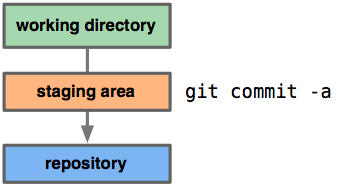
\includegraphics[width=\textwidth]{img/commitall}
        \caption[format=empty]{Quelle: \url{http://whygitisbetterthanx.com}}
      \end{figure}
    \end{column}
  \end{columns}
\end{frame}

\begin{frame}[fragile, allowframebreaks]{Historie betrachten}
  \begin{itemize}
    \item Historie in umgekehrt chronologischer Reihenfolge
    \begin{lstlisting}
$ git log
    \end{lstlisting}
  \begin{lstlisting}[frame=single]
commit ebae10784096e1ce3c2d4a8f2dd4cff32edfeaa0
Author: Wolfgang Silbermayr <wolfgang@example.com>
Date:   Sat Mar 19 17:38:35 2011 +0100

    %*\textcolor{darkgreen}{Add git-transport image}*)

commit 7198128a60a2c5b20d428722fa0341e0aaaae206
Author: Florian Preinstorfer <florian@example.com>
Date:   Sat Mar 19 17:27:12 2011 +0100

    %*\textcolor{darkgreen}{add hosting and collaboration frame}*)
  \end{lstlisting}
  \framebreak

    \item Git log erlaubt verschiedene Formatierungsoptionen
    \item Beispiel:
    \begin{lstlisting}
$ git log --pretty=format:'%h : %s' --topo-order --graph
    \end{lstlisting}
  \end{itemize}
  \begin{lstlisting}[frame=single]
*   ade7f24 : %*\textcolor{darkgreen}{Merge branch 'master' of gitorious.org:valug/git-slides}*)
|\  
| * 0bb70f1 : %*\textcolor{darkgreen}{change colors; add caption}*)
| * eaf4a3b : %*\textcolor{darkgreen}{use color in git status listing}*)
| *   808256f : %*\textcolor{darkgreen}{Merge branch 'master' of gitorious.org:valug/git-slides}*)
| |\  
| * | e63e26a : %*\textcolor{darkgreen}{add status file}*)
* | | 714815a : %*\textcolor{darkgreen}{Add branching commands}*)
| |/  
|/|   
* | 1ad271e : %*\textcolor{darkgreen}{Some special cases for diff lstlisting highlighting}*)
  \end{lstlisting}
\end{frame}

\begin{frame}[allowframebreaks]{Grafische git Tools}
  \begin{columns}
    \begin{column}{0.56\textwidth}
      \begin{figure}
        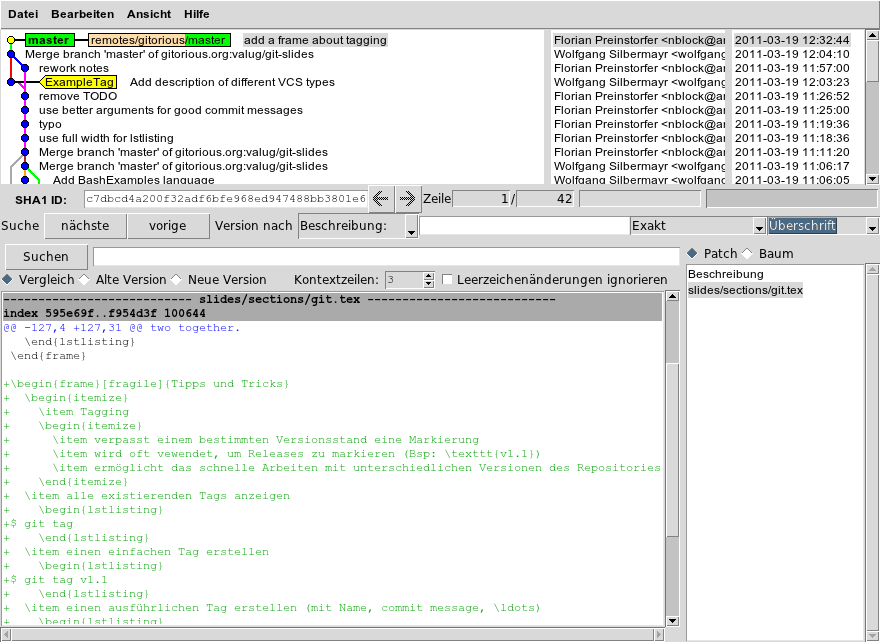
\includegraphics[width=\textwidth]{img/gitk}
        \caption{\href{http://www.kernel.org/pub/software/scm/git/docs/gitk.html}{gitk}}
      \end{figure}
    \end{column}
    \begin{column}{0.56\textwidth}
      \begin{figure}
        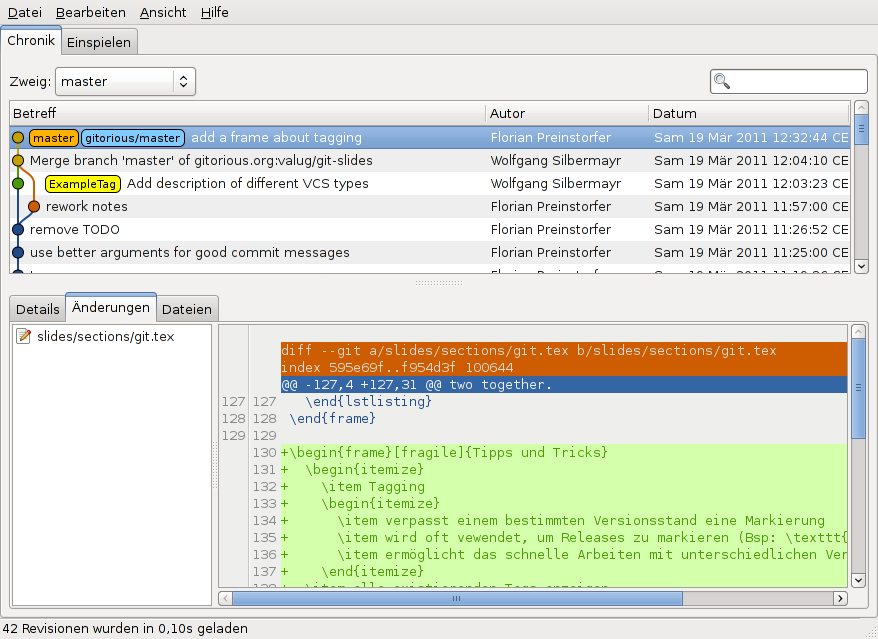
\includegraphics[width=\textwidth]{img/gitg}
        \caption{\href{http://trac.novowork.com/gitg}{gitg}}
      \end{figure}
    \end{column}
  \end{columns}
  
  \begin{columns}
    \begin{column}{0.56\textwidth}
      \begin{figure}
        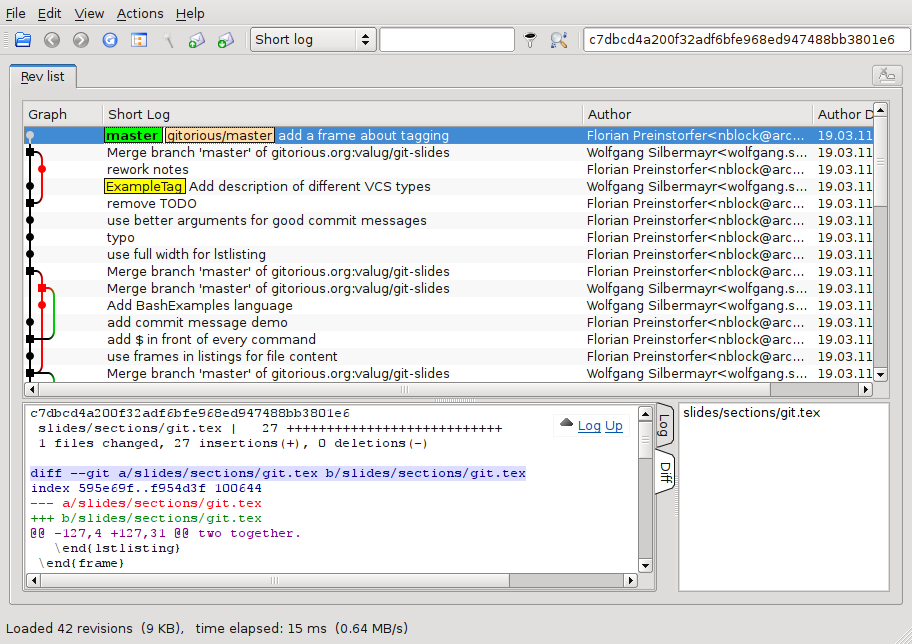
\includegraphics[width=\textwidth]{img/qgit}
        \caption{\href{http://sourceforge.net/projects/qgit}{qgit}}
      \end{figure}
    \end{column}
    \begin{column}{0.56\textwidth}
      \begin{figure}
        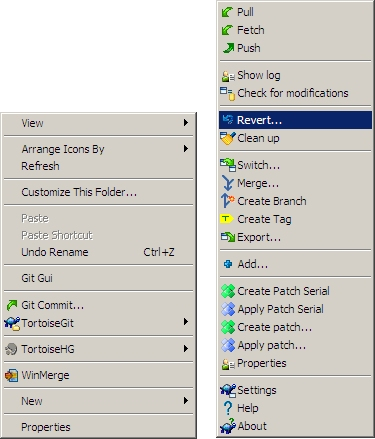
\includegraphics[width=0.61\textwidth]{img/tortoisegit}
        \caption{\href{http://code.google.com/p/tortoisegit}{tortoisegit}}
      \end{figure}
    \end{column}
  \end{columns}
\end{frame}

\begin{frame}[fragile, allowframebreaks]{Tipps und Tricks}
  \begin{itemize}
    \item Keine temporären Dateien in das git Repository aufnehmen
    \begin{itemize}
      \item Erschwert das effiziente Arbeiten mit git
      \item Bläht das Repository unnötig auf
    \end{itemize}
  \end{itemize}
  \begin{lstlisting}[frame=single, caption=Inhalt der Datei .gitignore]
*.swp       #alle swp Dateien
doc/*.aux   #alle aux Dateien im Verzeichnis doc/
tmp/**/*    #alle Dateien im Verzeichnis tmp/
  \end{lstlisting}
  \framebreak

  \begin{itemize}
    \item „Gute“ commit messages \ldots
    \begin{itemize}
      \item Vereinfachen die Zusammenarbeit
      \item Ermöglichen das schnelle Verfolgen von Änderungen
    \end{itemize}
  \end{itemize}
  \begin{lstlisting}[frame=single,caption={Quelle: \url{http://tbaggery.com/2008/04/19/a-note-about-git-commit-messages.html}}]
Short (50 chars or less) summary of changes

More detailed explanatory text, if necessary.  Wrap it to about 72
characters or so.  In some contexts, the first line is treated as the
subject of an email and the rest of the text as the body.  The blank
line separating the summary from the body is critical (unless you omit
the body entirely); tools like rebase can get confused if you run the
two together.
  \end{lstlisting}
  \framebreak

  \begin{itemize}
    \item Tagging
    \begin{itemize}
      \item Verpasst einem bestimmten Versionsstand eine Markierung
      \item Wird oft vewendet, um Releases zu markieren (Bsp: \texttt{v1.1})
      \item Ermöglicht das schnelle Arbeiten mit unterschiedlichen Versionen des Repositories
    \end{itemize}
  \item Alle existierenden Tags anzeigen
    \begin{lstlisting}
$ git tag
    \end{lstlisting}
  \item Einen einfachen Tag erstellen
    \begin{lstlisting}
$ git tag v1.1
    \end{lstlisting}
  \item Einen ausführlichen Tag erstellen (mit Name, commit message, \ldots)
    \begin{lstlisting}
$ git tag -a v1.1
    \end{lstlisting}
  \item Einen ausführlichen, mit GPG signierten, Tag erstellen
    \begin{lstlisting}
$ git tag -s v1.1
    \end{lstlisting}
  \end{itemize}
\end{frame}

% vim: tabstop=2 expandtab shiftwidth=2 softtabstop=2 autoindent


\begin{frame}{Referenzen}
\begin{description}
  \item[git:] \url{http://git-scm.com}
  \item[progit:] \url{http://progit.org}
\end{description}
\end{frame}

\begin{frame}[plain]
  \begin{center}
    \vspace{1cm}
    Danke!
    \vspace{3cm}
    \begin{figure}[!b]
      
\includegraphics[scale=0.5]{img/by-sa}
    \end{figure}
    \tiny{This work is licensed under the Creative Commons Attribution-ShareAlike 3.0 Austria license (CC-BY-SA).}
\end{center}
\end{frame}
\end{document}

% vim: tabstop=2 expandtab shiftwidth=2 softtabstop=2 autoindent
